\chapter{Implementierung eines Prototypen}\label{chap:implementation}

In diesem Kapitel wird die Entwicklung eines auf dem zuvor ausgearbeiteten Konzept basierten Prototypen beschrieben. Dieser Prototyp enthält nicht alle im Konzept beschriebenen Anforderungen und befindet sich auch nicht in einem finalen Entwicklungsstadium, kann aber mit weiteren Entwicklungsressourcen als Grundlage für eine finale Implementierung genutzt werden. Er soll zeigen, wie sich das entworfene Konzept umsetzen lässt und die darin benutzten Technologien miteinander interagieren.

\section{Tool zum Parsen der vorhandenen UI-Struktur}
Wie in Kapitel~\ref{chap:concept} beschrieben müssen die Dateien welche das momentane UI-Layout enthalten in ein web-freundlicheres Format (JSON) übersetzt werden. Bei diesem Schritt ist es auch direkt möglich Informationen die zukünftig nicht mehr benötigt werden nicht mit zu übernehmen und andere Informationen in eine optimalere Struktur zu überführen. Für diesen Zweck wurde ein kleines Hilfstool in C\# geschrieben, welches sowohl die ``.dli''-Datei der Detailansicht als auch die ``.vlc''-Datei der Übersichtsliste einer einzelnen cRM-Ansicht als Input erhält und daraus eine ``.json''-Datei mit allen benötigten Informationen erstellt. Um die Anpassbar- und Wiederverwendbarkeit des Tools zu maximieren wurde das \textbf{Visitor-Pattern} \fixme{Erklärung?} angewandt. In Abbildung~\ref{fig:web-conv_file-tree} ist der Aufbau des Tools erkennbar.

\begin{figure}
    \centering
    \captionsetup{justification=centering}
    \frame{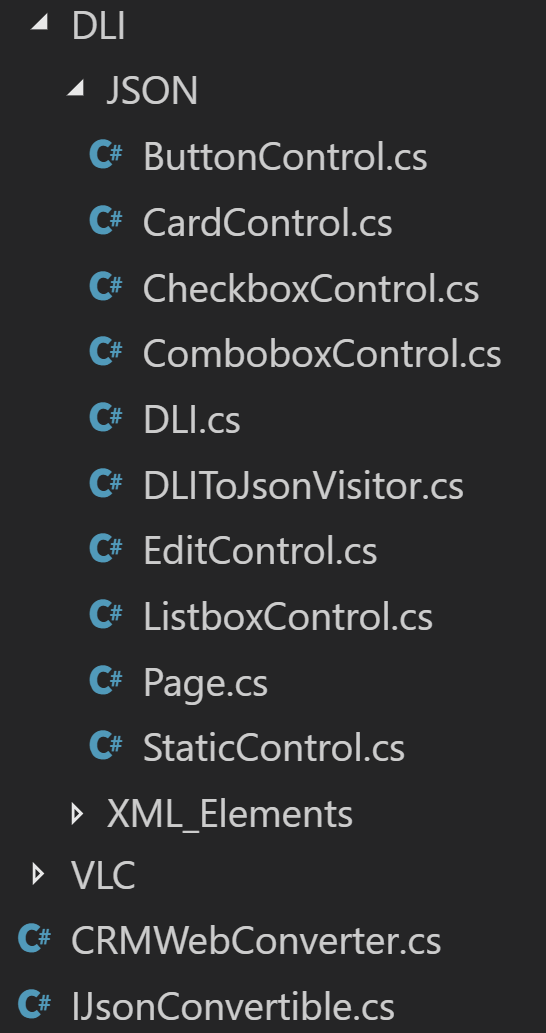
\includegraphics{figures/web-converter_file-tree.png}}
        \caption{Datei-Struktur des Konvertierungstools}\label{fig:web-conv_file-tree}
\end{figure}

Zunächst wird für jedes einzulesende Token (XML-Element) eine eine Klasse vom \textit{``Acceptor''}-Interface (\textit{IDLIAcceptor} / \textit{IVLCAcceptor}) abgeleitet, dieses Interface enthält eine einzige Methode \textit{``Apply''}, welche einen Visitor (\textit{IDLIVisitor} / \textit{IVCLVisitor}) übergeben bekommt. Die jeweiligen Token-Klassen werden mit dem von ihnen verwalteten XML-Element (\textit{XElement}) initialisiert. Wie im Quellcodeauszug~\ref{lst:pageelement_init} anhand der Klasse \textit{``PageElement''} beispielhaft zu sehen werden aus diesem XML-Element die relevanten Informationen über das Element selbst (Name und Metadaten) und dessen verschachtelte Kinder-Elemente (Liste von Controls) ausgelesen.

\lstinputlisting[language={[Sharp]C},label={lst:pageelement_init},caption={Initialisierung der PageElement-Klasse}]{code/chapter_005_pageelement_init.cs}

Nachdem die Informationen der XML-Datei auf diese Art und Weise in ihre einzelnen Token-Instanzen übersetzt wurden wird die \textit{Apply}-Methode, zu sehen in Quellcodeauszug~\ref{lst:dialogelement_apply}, des zentralen Tokens (\textit{DialogElement}) mit einer Visitor-Instanz aufgerufen. Der Visitor erhält als Parameter eben diese Instanz und extrahiert alle für ihn relevanten Informationen. Anschließend ruft er rekursiv die \textit{Apply}-Methoden der Kinder-Token auf und liest auch aus diesen die relevanten Informationen aus. Diese Aufrufe sind im Quellcodeauszug~\ref{lst:json-visitor_visit-methods} zu sehen. Nachdem alle Tokens vollständig besucht wurden können die gewonnenen Daten als JSON-String ausgegeben werden.

\lstinputlisting[language={[Sharp]C},label={lst:dialogelement_apply},caption={Apply-Methode der DialogElement-Klasse}]{code/chapter_005_dialogelement_apply.cs}

\lstinputlisting[language={[Sharp]C},label={lst:json-visitor_visit-methods},caption={Besuchen von und Extrahieren relevanter Informationen aus XML-Tokens durch den JSON-Visitor}]{code/chapter_005_json-visitor_visit-methods.cs}

Die Flexibilität dieser Architektur, welche in der Abbildung~\ref{fig:web-conv_class-diagramm} nochmals übersichtlich als Klassendiagramm dargestellt wird, ist ebenso daran zu erkennen, dass der einzige Unterschied beim Auslesen von Detailansicht-Datei und Übersichtslisten-Datei in der Implementierung der Interfaces besteht. Sowohl \textbf{Acceptor}- als auch \textbf{Visitor}-Klassen können sehr leicht einzeln angepasst oder ersetzt werden. Ebenso ist es möglich weitere Tokens, welche eventuell zu einem späteren Zeitpunkt benötigt werden, aus den XML-Dateien auszulesen, indem man weitere \textbf{Acceptor}- und \textbf{Visitor}-Implementierungen hinzufügt.

\begin{figure}
    \centering
    \captionsetup{justification=centering}
    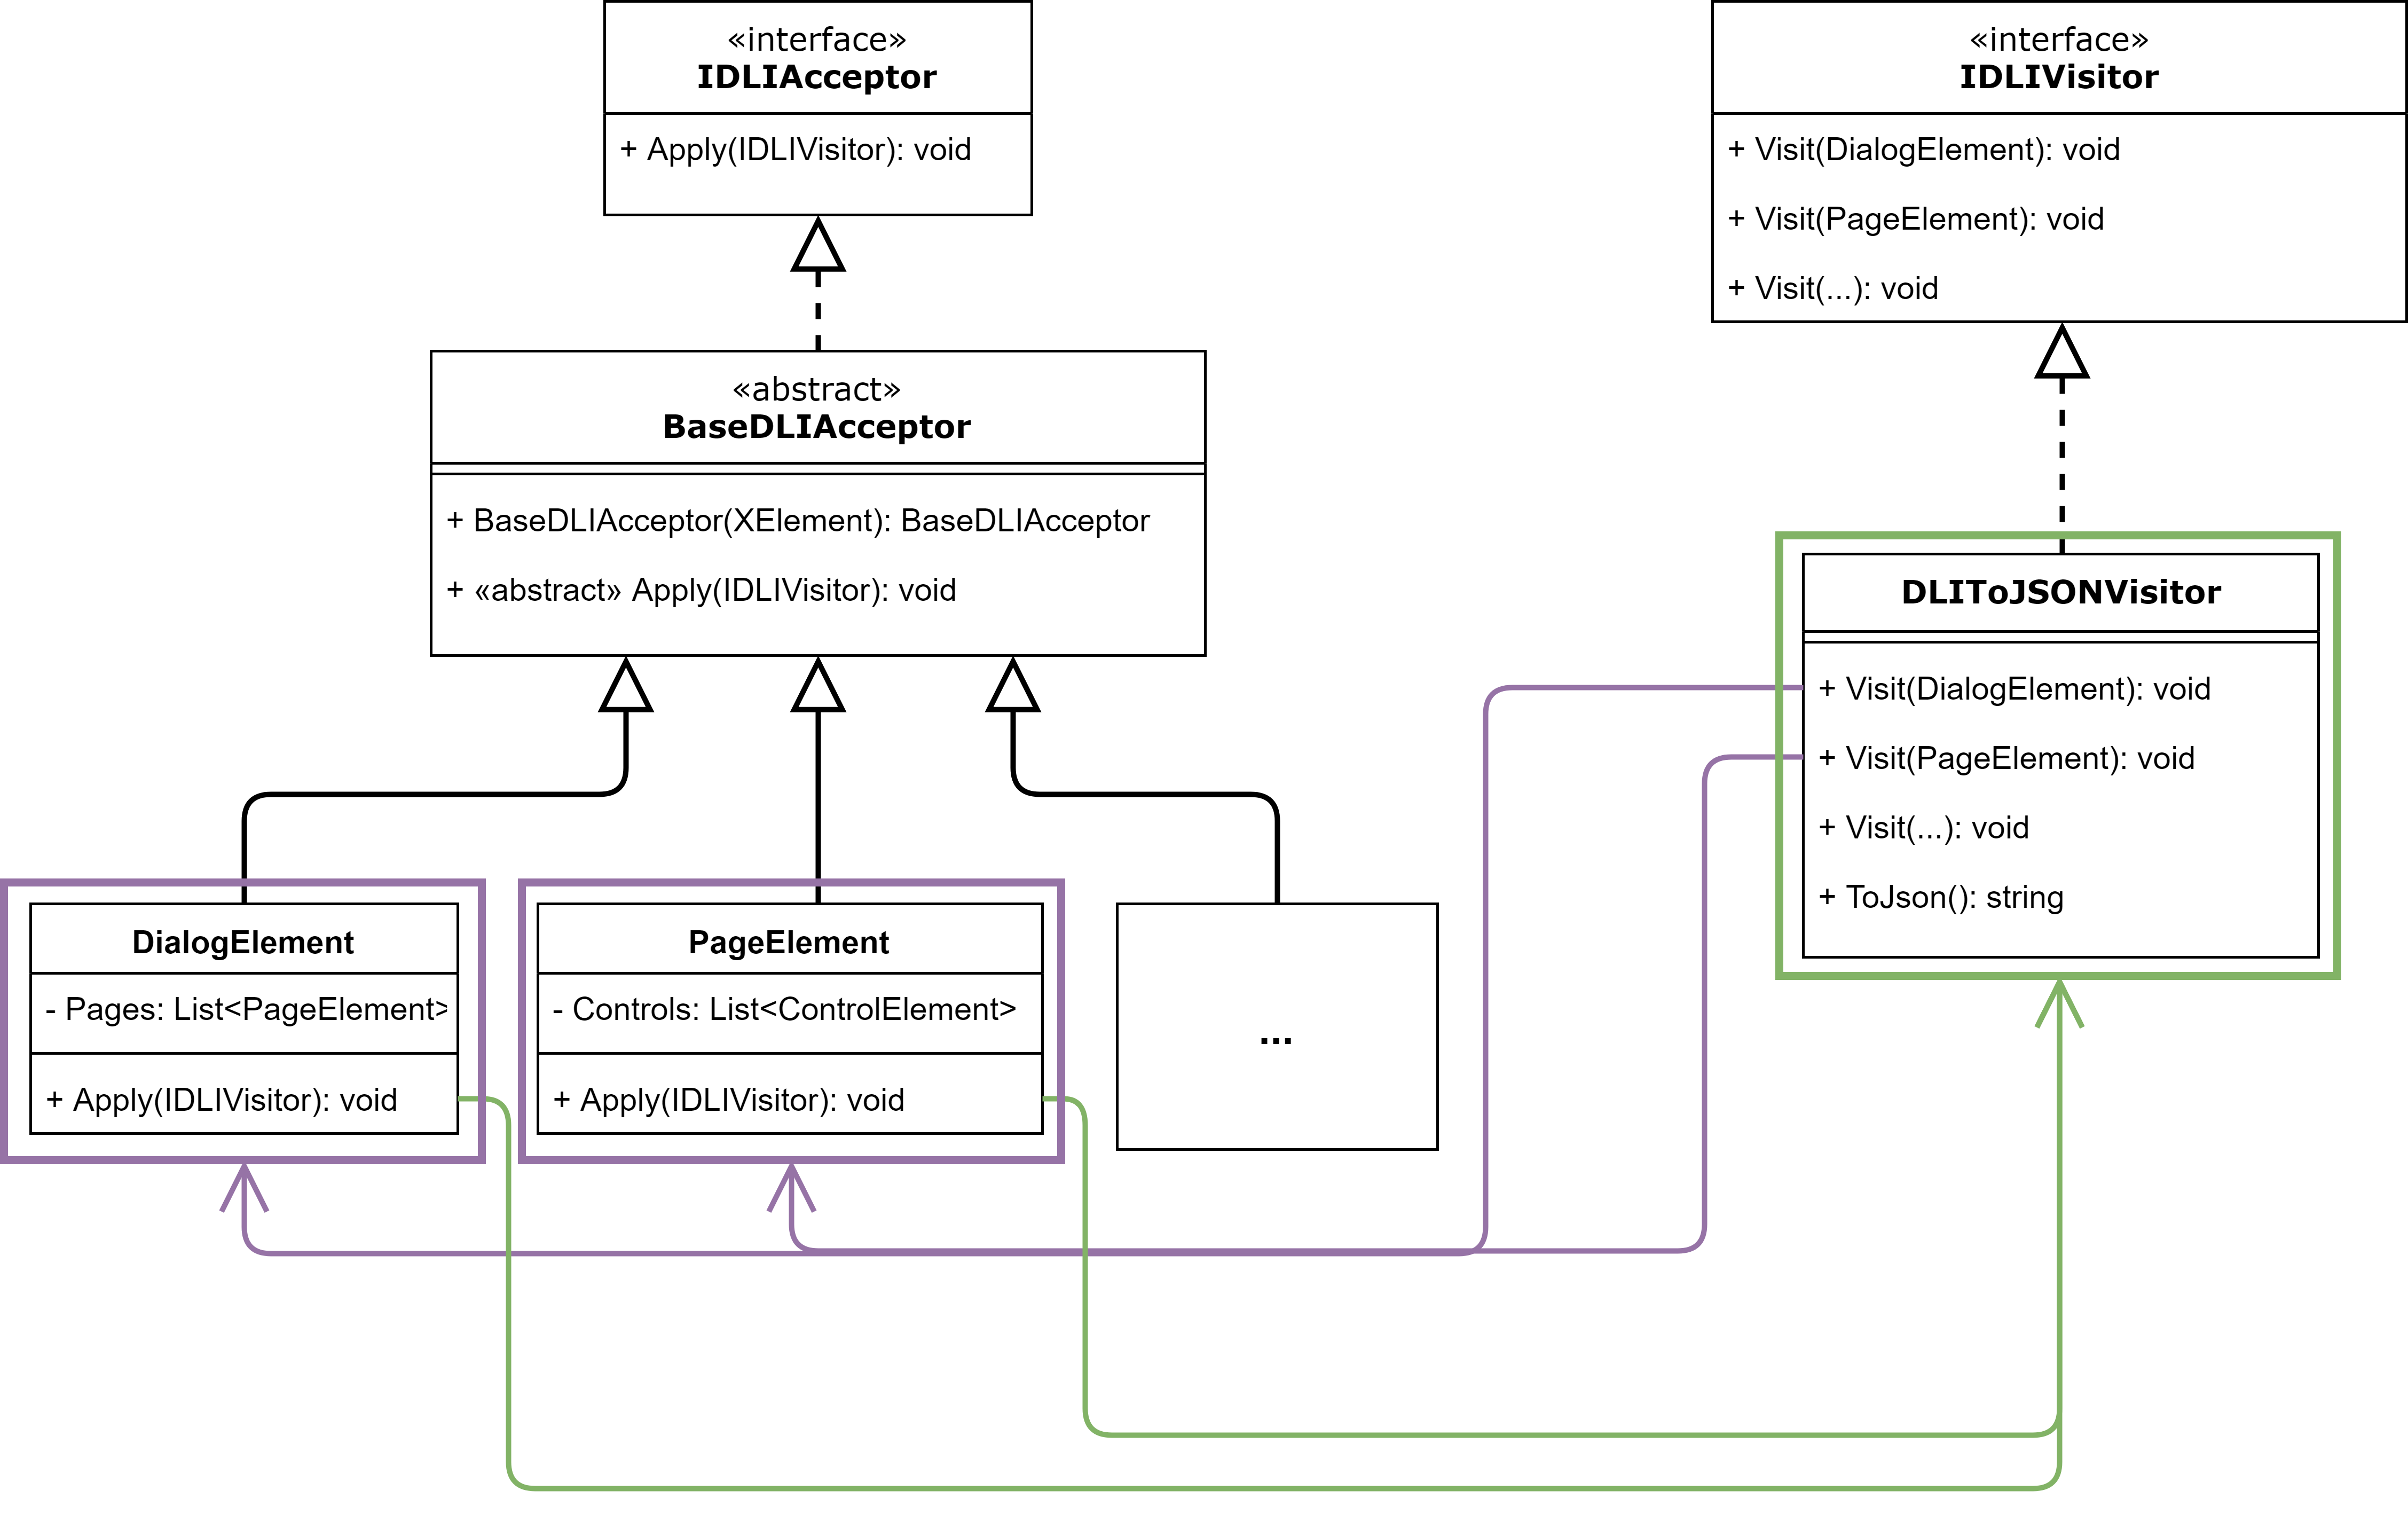
\includegraphics[width=\textwidth]{figures/web-converter_class-diagramm.png}
        \caption{Klassendiagramm der Visitor-Struktur des Konvertierungstools}\label{fig:web-conv_class-diagramm}
\end{figure}

Der Input und das Endergebnis in Form eines vom GraphQL-Server direkt verwertbaren JSON-Dokument ist in den beiden Quellcodeauszügen~\ref{lst:xml_input} und \ref{lst:json_output} anhand eines kleines Auszuges ersichtlich. \fixme{vollständigeres beispiel und erklärung?}

\fixme{Syntaxhighlighting:}
\lstinputlisting[language={XML},caption={XML-Input},label={lst:xml_input}]{code/chapter_005_xml_input.xml}
\lstinputlisting[caption={JSON-Ergebnis},label={lst:json_output}]{code/chapter_005_json_output.json}

\section{Webseite}

\subsection{CRA-Skelett}
\subsection{React-Komponenten}

\subsection{Benutzung der Komponenten}
\subsection{Storybook und Tests}
\subsection{GraphQL-Mock-Server und Resolver}

% EINFACHES (wenig Elemente), ABER KOMPLETTES BSP für jetzige UI -> neue UI
